% !TEX TS-program = pdflatex
% !TEX encoding = UTF-8 Unicode

% This is a simple template for a LaTeX document using the "article" class.
% See "book", "report", "letter" for other types of document.

\documentclass[12pt]{article} % use larger type; default would be 10pt

\usepackage[utf8]{inputenc} % set input encoding (not needed with XeLaTeX)

%%%%\usepackage[document]{ragged2e} 

%%% Examples of Article customizations
% These packages are optional, depending on whether you want the features they provide.
% See the LaTeX Companion or other references for full information.

%%% PAGE DIMENSIONS
\usepackage{geometry} % to change the page dimensions
\geometry{letterpaper} % or letterpaper (US) or a5paper or....
\geometry{margin=1in} % for example, change the margins to 2 inches all round
% \geometry{landscape} % set up the page for landscape
%   read geometry.pdf for detailed page layout information

\usepackage{graphicx} % support the \includegraphics command and options
\graphicspath{
{figs/ipe/}
}
% \usepackage[parfill]{parskip} % Activate to begin paragraphs with an empty line rather than an indent

%%% PACKAGES
\usepackage{booktabs} % for much better looking tables
\usepackage{array} % for better arrays (eg matrices) in maths
\usepackage{paralist} % very flexible & customisable lists (eg. enumerate/itemize, etc.)
\usepackage{epstopdf}
\epstopdfsetup{suffix = {}}
\usepackage{siunitx}
\sisetup{inter-unit-product = \cdot}
\usepackage{verbatim} % adds environment for commenting out blocks of text & for better verbatim
\usepackage{subfig} % make it possible to include more than one captioned figure/table in a single float
% These packages are all incorporated in the memoir class to one degree or another...

\usepackage{caption}        %Allows modification of captions
% \usepackage{indentfirst}    %Allows for indenting first paragraphs


\usepackage{hyperref}

% \usepackage{easyReview}

%%% HEADERS & FOOTERS
\usepackage{fancyhdr} % This should be set AFTER setting up the page geometry
\pagestyle{fancy} % options: empty , plain , fancy
\renewcommand{\headrulewidth}{0pt} % customize the layout...
\lhead{}\chead{}\rhead{}
\lfoot{}\cfoot{\thepage}\rfoot{}

%%% SECTION TITLE APPEARANCE
\usepackage{sectsty}
\usepackage{tikz}
\usepackage[framemethod=TikZ]{mdframed}
\usepackage{enumerate}
\allsectionsfont{\sffamily\mdseries\upshape} % (See the fntguide.pdf for font help)
% (This matches ConTeXt defaults)

%%% ToC (table of contents) APPEARANCE
\usepackage[nottoc,notlof,notlot]{tocbibind} % Put the bibliography in the ToC
\usepackage[titles,subfigure]{tocloft} % Alter the style of the Table of Contents


\usepackage[colorinlistoftodos]{todonotes}
\usepackage{soul}

\renewcommand{\cftsecfont}{\rmfamily\mdseries\upshape}
\renewcommand{\cftsecpagefont}{\rmfamily\mdseries\upshape} % No bold!

\newcommand{\HRule}{\rule{\linewidth}{0.5mm}} % Command to make the lines in the title page

%%% END Article customizations

%%% The "real" document content comes below...

\title{
    \begin{center}
        \href{http://www.bradley.edu}{
\includegraphics[height=1in]{figs/logoBU1-Print}}
        \vskip10pt
        \HRule \\[0.4cm]
        {\Huge \bfseries Hardware-in-the-Loop Plant Modeling for Autonomous Vehicle \\\Large Project Statement and Functional Requirements}\\[0.4cm] % Degree
        \HRule \\[0.4cm]
    \end{center}
    }
\author{Hannah Grady and Nicholas Nauman \\ \underline{Advisor}: Dr. Suruz Miah}

%\date{} % Activate to display a given date or no date (if empty),
         % otherwise the current date is printed 
         
% \setlength{\parindent}{4em} % this should indent paragraphs

\setlength{\marginparwidth}{2cm}

\begin{document}
\maketitle

% \newpage
% \tableofcontents % Table of contents
\newpage % Start lab look on a new page

\section{Project Description}
Autonomous vehicles are being developed by many companies for commercial and/or personal use. These autonomous vehicles would allow companies to continue crucial deliveries or transports of their products even if there is a shortage of drivers. Also, autonomous vehicles have the ability to make roads safer for drivers and pedestrians alike. To control autonomous vehicles, accurate models of six main vehicle subsystems must be created so controllers can be developed to reliably manage the system.

There are six main subsystems - a steering model, an acceleration model, a brake
model, a shifting model, a speed model, and a cruise model - that must be
modeled to get an accurate representation of how the vehicle should be
controlled. We will be modeling these six subsystems for a Lexus platform using
the System Identification Toolbox from Matlab. The first subsystem we will model is the steering model, and then we will move onto the other subsystems. There are controllers in place to control the Lexus vehicle platform, but the reliability of these controllers is lower than expected. The scope of this project includes developing models for each subsystem so Autonomous Stuff can implement controls that improve the reliability of the vehicle platform. These models will be used by AutonomouStuff for their Hardware-in-the-Loop (HIL) testing. 

%------------------------------------------------

\section{Literature}
\label{sec:Literature}

Researchers in~\cite{Adnan2010} show how a system with small non-linearities can
be modeled using Matlab's System Identification Toolbox. Since the researchers
were able to model their system successfully, that indicates that we should be
able to model our steering model with its small non-linearities caused by very
small steering angles as well. Another method for modeling small non-linearities
is introduced by the authors in~\cite{Saruchi2015} using a Steer-By-Wire method
as the model for the steering system. With this model, a composite nonlinear
feedback (CNF) PID controller can be implemented to control the steering system
even for small turning angles. Another option for modeling the steering system
is using a third order ARMAX model as proposed by~\cite{Li1999}. Using this
model, traditional analysis methods can be used to develop a model and
controller. Any concerns that modeling the vehicle components using the System
Identification Toolbox will produce inaccurate results are addressed by
~\cite{Donjaroennon2021}. Using input and output signals, they were able to come
up with a model that had a best fit percentage of 95.1\%. With these options for
modeling automotive systems, we can carry out our project knowing that the
models we produce will be accurate.

%------------------------------------------------
\section{System Architecture}
\subsection{System Block Diagram}
The Lexus car platform is comprised of six main subsystems - a steering model,
an acceleration model, a brake model, a shifting model, a speed model, and a
cruise model. The system, as a whole, will be taking into consideration
obstacles around it while the vehicle traverses a predetermined route. For the
system to be able to accomplish this reliably, the six main subsystems must be
precisely modeled, especially the steering subsystem. A block diagram of the
vehicle steering model is shown in \autoref{fig:sysBlockDiag}. %
%
\begin{figure}[h]
    \centering
    \captionsetup{justification=centering, margin=3cm}
    \includegraphics[width=3.5in]{figs/inkscape/steeringModelArchitecture}
    \caption{Block Diagram of the Vehicle Steering Model.}
    \label{fig:sysBlockDiag}
\end{figure}
%

\subsection{System Inputs and Outputs}
\subsubsection{Inputs}

\todo[inline]{For the steering model, is it a single input (torque voltage) and multiple output system?}
\begin{itemize}
    \item Steering Model
    \begin{itemize}
    		\item Torque Voltages
    		\begin{itemize}
    			\item Desired Steering Wheel Angle
    			\item Actual Steering Wheel Angle
    		\end{itemize}
    \end{itemize}
    \item Acceleration Model
    \begin{itemize}
    		\item Acceleration Pedal Voltages
    \end{itemize}
    \item Brake Model
    \begin{itemize}
    		\item Brake Pedal Pressure Voltages
    		\item Brake Pedal Stroke Voltages 
    		\item Brake Pedal On/Off Switch
    \end{itemize}
    \item Shift Model
    \begin{itemize}
    		\item Desired Shift Gear
    \end{itemize}
    \item Speed Model
    \begin{itemize}
    		\item Acceleration Pedal Position
    		\item Brake Pedal Position
    		\item Shifter Actual Gear
    \end{itemize}
    \item Speed Control Model
    \begin{itemize}
    		\item Desired Vehicle Speed
    \end{itemize}
\end{itemize}

\subsubsection{Outputs}

\begin{itemize}
    \item Steering Model
    \begin{itemize}
    		\item Wheel Angle
    		\item Actual Steering Wheel Angle
    \end{itemize}
    \item Acceleration Model
    \begin{itemize}
    		\item Acceleration Pedal Position
    \end{itemize}
    \item Brake Model
    \begin{itemize}
    		\item Brake Pedal Position
    		\item Brake Pressed
    \end{itemize}
    \item Shift Model
    \begin{itemize}
    		\item Shifter Actual Gear
    \end{itemize}
    \item Speed Model
    \begin{itemize}
    		\item Vehicle Speed
    \end{itemize}
    \item Speed Control Model
    \begin{itemize}
    		\item Vehicle Speed
    \end{itemize}
\end{itemize}

%------------------------------------------------
\section{Requirements and Specifications}
\subsection{Requirements}
The vehicle platform plant model will meet the following requirements:
\begin{itemize}
    \item The plant model should have an accurate model of the six main subsystems
    \item A HIL test bench can be developed from the plant models of the subsystems
    \item The steering model can handle very small steering angles
\end{itemize}

\subsection{Specifications}
Based on the requirements, the vehicle platform plant model must meet the following specifications:
\begin{itemize}
    \item The model of the steering subsystem should be modeled first as it is crucial to operation and has non-linearity considerations
    \item The remaining subsystems will be modeled individually 
    \item Our steering model will be designed to accommodate very small steering angles
\end{itemize}

%------------------------------------------------
\section{Other Considerations}
As we progress with this project, it is important that we take into consideration how this will affect others and make sure that we are holding ourselves to high ethical standards. 
\begin{itemize}
    \item Public Health: Autonomous vehicles can make roads safer, which can prevent accidents and driving fatalities and injuries. As a result, people will be able to live longer and healthier lives. By creating accurate models, we will help advance the development of autonomous vehicles and make this a reality. 
    \item Public Safety: This is a relevant concern, because the real world implementations of inaccurate models could be disastrous since it is a self-driving vehicle. We will address this by creating a rigorous test plan for our models. 
    \item Public Welfare: This factor is somewhat related to public safety and health in that we need to make sure that these vehicles are safe for people to use. How we will help ensure this in our project is the same as how we will ensure public safety, by making sure we throughly test our models. 
    \item Global Factors: Our work will be used to help advance the technology behind autonomous vehicles, but we will not have any control over how they will be used in society. Therefore, this factor is irrelevant the project. 
    \item Cultural Factors: This is irrelevant to this project. While our work will help with the development of autonomous vehicles, we do not have any control or impact over how they will be introduced within cultural boundaries.
    \item Social Factors: Advancing autonomous vehicle research could lead to them replacing those who drive for a living, such as taxi or Uber drivers. This is an important issue that needs to be addressed as autonomous vehicles become more widespread, but it is outside of the scope of our project. 
    \item Environmental Factors: By modeling the vehicle components using software, that means the vehicle will not have to be used as often for testing. Less vehicle use could potentially have a positive impact on the environment. 
    \item Business Factors: We must keep in mind the maintenance of developed software to control the vehicle based on updates to the control models. 
    \item Economic Factors: There is an increased cost associated with the specialized hardware which allows for the autonomy of the vehicle. However, this cost is justified to the consumer as it reduces the stress and time involved with driving a vehicle. 
\end{itemize}

%------------------------------------------------
\pagebreak
\bibliographystyle{IEEEtran}
\bibliography{bib/references.bib}
\end{document}

%%% Local Variables:
%%% mode: latex
%%% TeX-master: t
%%% End:
